\chapter{Methodology}
This chapter mainly discusses the methodology. First, we explain the data which we used. After that, the baseline method is elaborated. Lastly, we propose new data selection algorithms.
% Overall Data
% part2
% Metadata
% MGB Baseline

\section{Data}
% cite it here
For this internship, we used TV broadcasts downloaded from internet. 
\begin{itemize}
\item The audio files are taken from TV broadcasts over period of 1 April 2008 - 19 may 2008(7 weeks). Total duration of audio is 1,600 hours.
\item TV brodcast transcriptions(7 weeks closed captions) of the audio files are provided. The closed captions are close to what the audio says, but not exactly the same as the speakers of the audio said.
\item 640 million words of TV subtitles are given over the period of 1979-2013. In addition to that, the 640M subtitles are filtered to avoid overlap with the 7 weeks closed captions.
\end{itemize} 

We prepared two data sets: training set and development set. The training dataset has a total duration of 1600 hours of audio. To evaluate our model, we have a development set. To accelerate the acoustic model training,  we selected roughly 200 hours of data from the training set. Some metadata are provided in our data, such as: speaker id of the transcript, genre of the show, date and time of the show, as well as television channel where the show was aired. In addition, each segment has start and end time when the segment was shown in the TV broadcast. 

How to select 200 hours(train.200) and 100 hours(train.100) subset of data: 
\begin{enumerate}
\item The files in train.full were sorted by their size.
\item Select the biggest file out of 8 files.
\item Write the selected data into 200 training set file.
\end{enumerate}
Because the duration of train.full is more or less 1600 hours, 200 hours of data were obtained by using this random selection. 

\begin{center}
\begin{tabular}{ | c | c | c | c | c | c | c | }
\hline
No & Data set & \#shows & Duration(h) & Aligned speech (h) \\ \hline
1 & full training set & 2,193 & 1,580 & 1,197 \\ \hline
2 & dev.short & 12 & 8 & 6 \\ \hline
3 & train.200 & 274 & 193  & 149 \\ \hline
\end{tabular}
\end{center}

 After obtaining 200 hours of data, a 100 hours subset was created by selecting one from two files from 200 training set. The 200 hours and 100 hours training set are named as train.200 and train.100 respectively.


All files in full training set have closed captions. In contrast, all files in development set have closed captions as well as manually annotated human transcription. The transcript is manually and carefully annotated by human. Thus, the transcript is believed to be the closest transcription spoken by speakers in audio files.

%\begin{figure}
%\begin{subfigure}{.5\textwidth}
%\caption{AWD}
%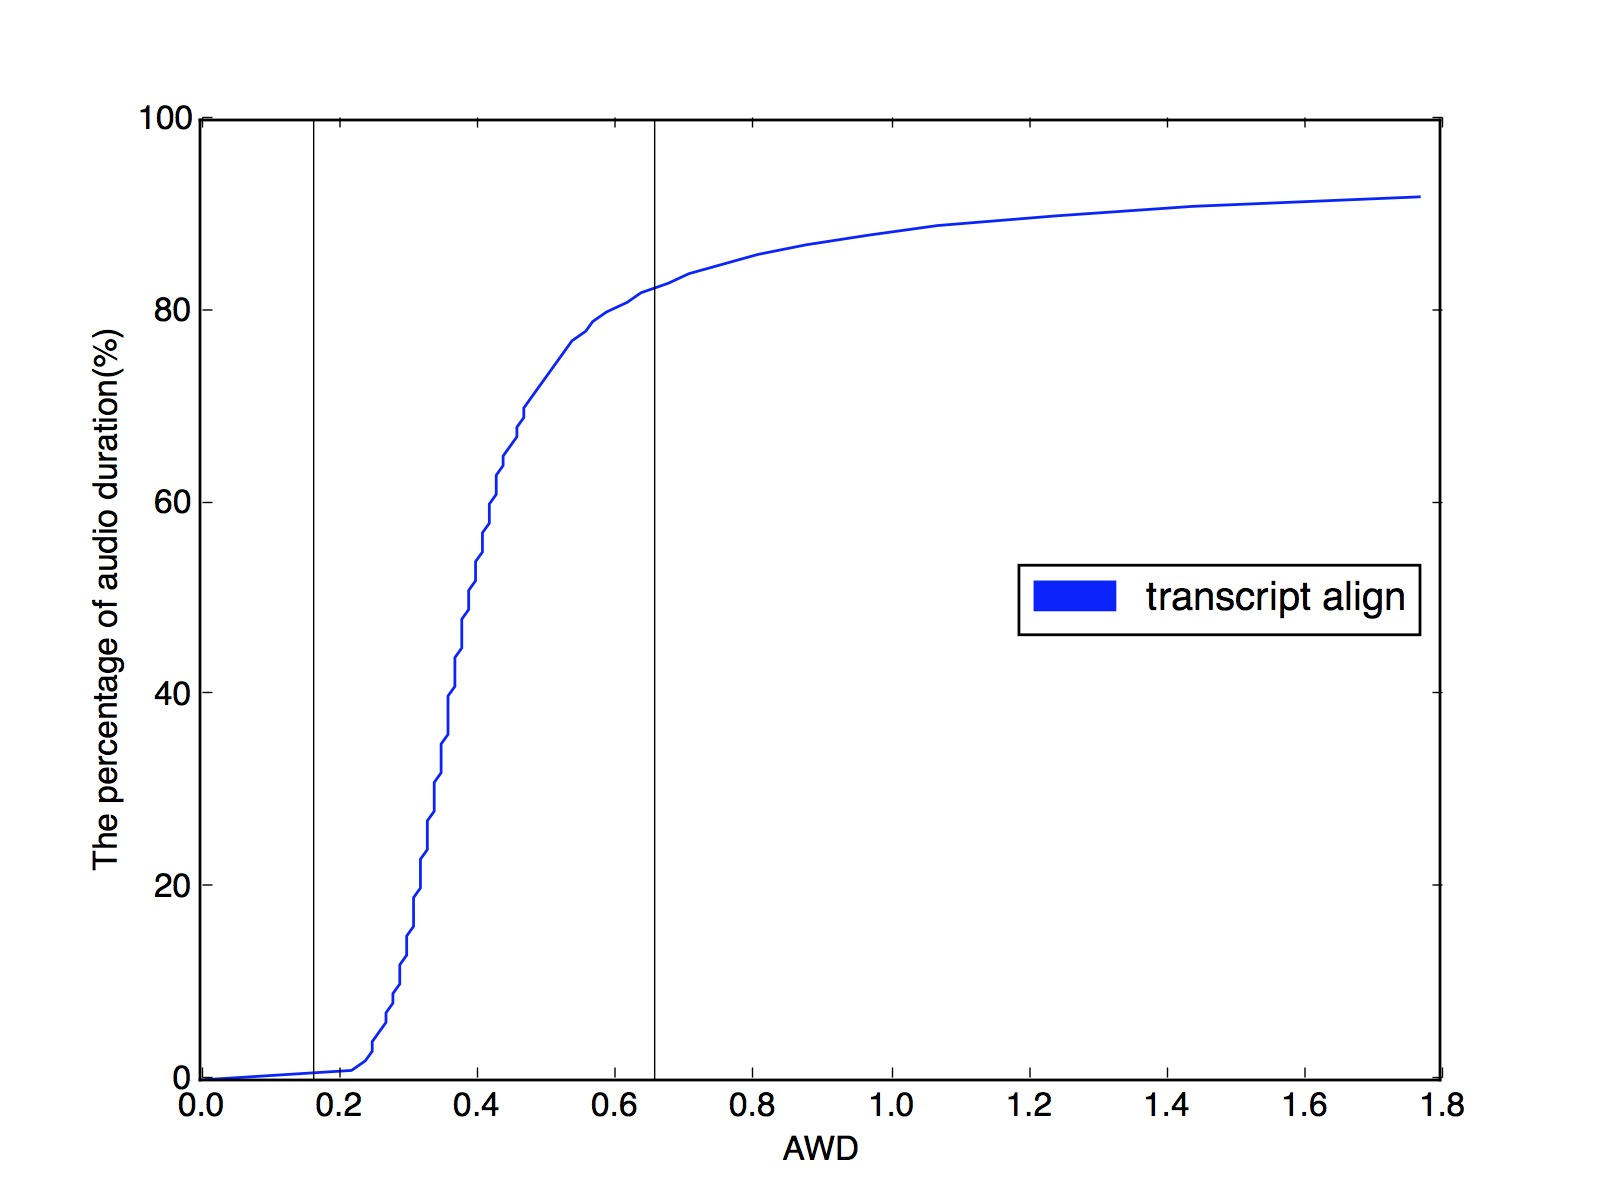
\includegraphics[scale=0.15]{awdAlign}
%\end{subfigure}
%\begin{subfigure}{.5\textwidth}
%\caption{WMER and PMER}
%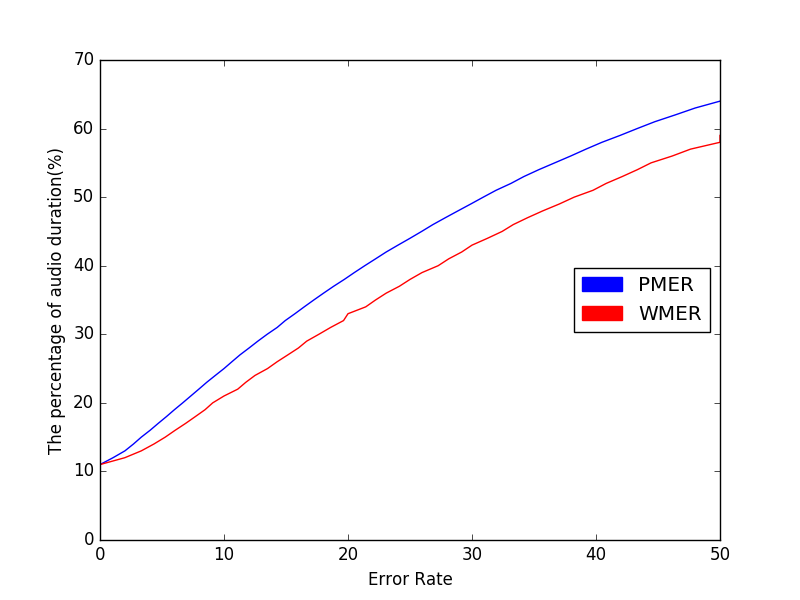
\includegraphics[scale=0.4]{pmerwmerAlign}
%\end{subfigure}
%\caption{Aligned transcription provided by MGB}
%\end{figure}

\begin{center}
\captionof{table}{Statistics of train.200 per genre}
\begin{tabular}{ | c | c | c | c|}
\hline
\textbf{Genre} & \textbf{\#shows}  & \textbf{Duration(h)} & Aligned speech(h) \\ \hline \hline
advice & 40 & 26 & 22 \\ \hline
children & 51 & 19 & 14 \\ \hline
comedy & 19 & 8 & 6 \\ \hline
competition & 30 & 21 & 16 \\ \hline
documentary & 29 & 22 & 14 \\ \hline
drama & 20 & 14 & 10 \\ \hline
events & 24 & 38 & 29 \\ \hline
news & 61 & 42 & 37 \\ \hline
\end{tabular}
\end{center}

\begin{figure}
\caption{Bar chart of each genre from all training data and 200 hours training data}
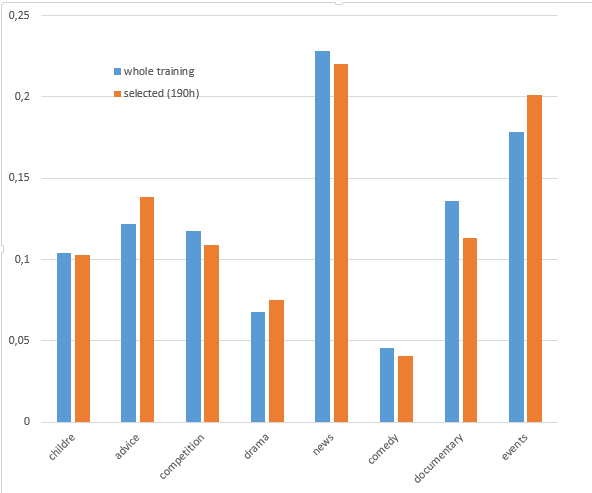
\includegraphics[scale=0.5]{barchartgenre}
\centering
\end{figure}


% Dataset
% explain dev.short, train.200, train.full
% transcript align, transcript lsdecode, transcript human


\section{Baseline model}
This section explains the baseline data selection technique which is inspired from Woodland \cite{Woodland2015}. First, we explain how to evaluate whether data selection works well. Then, we elaborate the baseline algorithm. 



\subsection{Error rate and average word duration}
The standard evaluation of speech recognition is word error rate(WER). WER compares and counts the number of edits between the real transcription and the decoding result(the hypothesis transcription which is produced by the speech recognizer). The first step to calculate WER is by computing the number of edits with minimum edit distance algorithm. The algorithm produces the number of substitution, insertion, and deletion.  Then, word error rate can be calculated as following:
\begin{equation}
\textrm{Word error rate} = 100 \times \frac{\textrm{Insertion} + \textrm{Substitution} + \textrm{Deletion}}{\textrm{Total words in correct transcript}}
\end{equation}

Phone error rate(PER) is a metric which compares the hypothesis transcriptions and the real transcriptions in phone level. Instead of comparing words(calculating WER), we need to compare phone in data selection problem. The main reason is we want to improve the acoustic model which outputs a sequence of hypothesized phones. 

When selecting the subset of data, we compared the closed captions and the output of speech recognition. To avoid confusion with WER and PER(error rate between the hypothesized transcriptions and the real transcriptions), we used term word matched error rate(WMER) and phone matched error rate(PMER), which is an error rate between the closed captions and the decoding results in word and phone level respectively.

One of the standard framework of running minimum edit distance and calculating error rate is sclite. sclite is able to do alignment and calculate error rate. Moreover, it provides some statistic summary, e.g. total insertion, total deletion, overall error rate, etc, and calculate error rate for each speaker. It also provides insertion, deletion, and substitution for each segment which later can be used to calculate WMER and PMER for each segment.  

%\subsection{Cambrige method}
% explain cambridge method here


\subsection{Our baseline method}


Our baseline was inspired from the Cambridge method \cite{Woodland2015}. As shown in the picture \ref{fig:LandscapeDataPipeline}, our baseline technique has two pipelines: data selection and evaluation. Data selection pipeline is to select the best subset of data, while the evaluation pipeline is to measure how good the selected data is. 

The data selection pipeline works as following:
\begin{enumerate}
\item Train an acoustic model(AM.100-v0) on 100 hours of training data(train.100)
\item Build a language model(e.g. LM.200.1e-9) from 200 hour transcriptions. This language model was built from closed captions of train.200. Then, the language model is pruned by $10^{-9}$. In other word, if the probabilities of N-Gram word sequence is less than $10^{-9}$, they will be excluded. We will elaborate the language model in the next section. 
\item By utilizing the acoustic model(AM.100-v0),  the language model(LM.200.1e-9), and a lexicon(e.g. Lexicon.200), recognize the development set(8 hours dev set) to know the overall PER and WER. Our lexicon is from Combilex British English lexicon. Lexicon.200 is a subset of Combilex lexicon which consists of words in the 200-hour training set(train.200).
\item By using the same acoustic model(AM.100-v0), language model, and lexicon recognize the 200 hour training set. From the recognition process, calculate PMER(phone matched error rate), WMER(word matched error rate), and AWD(average word duration) of each segment. 
\item Sort segments according to its PMER. Choose 100 hour segments with top PMER value if the segments has AWD with range between 0.165 and 0.66.  This range follows the AWD range from the Cambridge method.
\item Train a new acoustic model(AM.100-v1) with the 100 hour data(100-v1). 
\item Utilizing AM.100-v1, LM.200, and Lexicon.200, recognize 200 hours data to get 100 hour data(100-v2). Retrain an acoustic model(AM.100v2) by using 100-v2 and re-recognize the 200 hour data. Reiterate the process of selecting(100-v3 and so on) and training data(AM.100v3 and so on) until no further improvement is found.
\end{enumerate}

When to stop the data selection pipeline? The answer is to utilize the evaluation pipeline. The evaluation pipeline will produce phone matched error rate(PMER) and word matched error rate(WMER). If WMER decreases in the next iteration, we continue our iteration; otherwise, we halt the iteration. 

\begin{sidewaysfigure}
	\clearpage 
	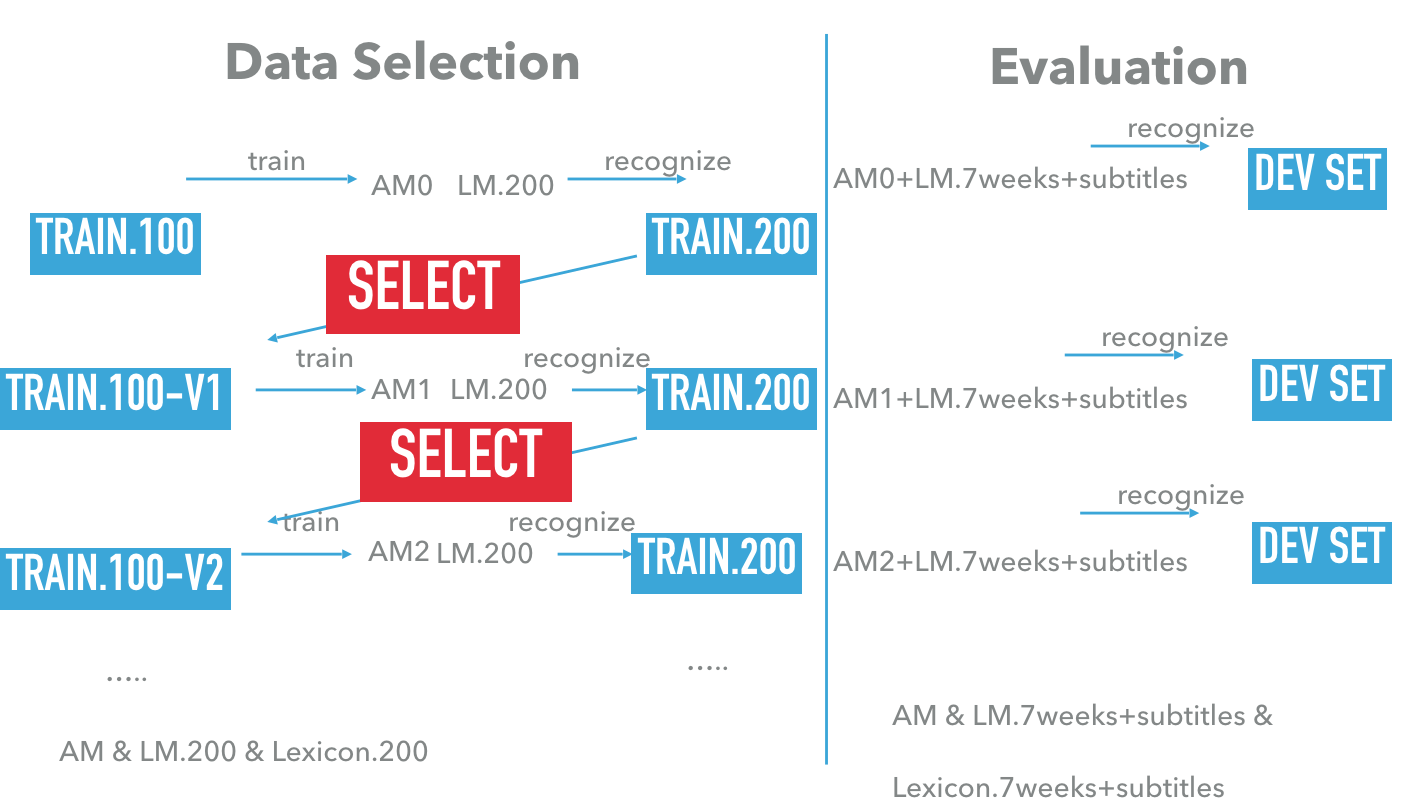
\includegraphics[width=\textwidth]{datapipeline}
    	\caption{Data selection pipeline}
    	\label{fig:LandscapeDataPipeline}
\end{sidewaysfigure}



\subsection{Language model}
This internship experimented with three different kinds of language model. All language models are based on four gram language model. 
\begin{enumerate}
\item LM.200 \\
This language model, named as LM.200, was produced from the closed captions of 200 hours training set(train.200). LM.200 was pruned by $10^{-9}$.  LM.200 was used for the baseline speech recognizer to select the "good" subset of data.

\begin{center}
\captionof{table}{Statistics of LM.200}
\begin{tabular}{ | c | c | c | }
\hline
\textbf{No.} & \textbf{File}  & \textbf{Information} \\ \hline \hline
1 & word.200 & 33,914 words \\  \hline
2 & LM.200 & uni-gram=33916 \\ 
 & & bi-gram=402299 \\ 
& & tri-gram=111868 \\  
& & 4-gram=64801 \\  \hline
3 & LM.200.1e-9 & ngram 1=33916 \\  
 & & ngram 2=402299 \\  
& & ngram 3=98566 \\  
& & ngram 4=51215 \\  \hline
\end{tabular}
\end{center}

\item LM.7weeks+subtitles.limited.1e-9 \\
A language model was generated from the closed captions of 7 weeks transcription and interpolated with a language model from the big TV subtitles with ratio 0.9/0.1. The language model was limited by top 160,000 frequent word list and pruned by $10^{-9}$ resulting in LM.7weeks+subtitles.limited.1e-9.  The language model and together with an acoustic model and a lexicon was utilized to compute error rate of the development set.

\begin{center}
\begin{tabular}{ | c | c | c | }
\hline
\textbf{No.} & \textbf{File}  & \textbf{Information} \\ \hline \hline
1 & word.160k & 160,000 words \\  \hline
2 & LM.7weeks & ngram 1=91836 \\
 & & ngram 2=1817881 \\
 & & ngram 3=980925 \\
 & & ngram 4=847736 \\  \hline
3 & LM.subtitles & ngram 1=756644 \\
 & & ngram 2=27144330 \\
 & & ngram 3=37162518 \\
 & & ngram 4=57912280 \\ \hline
4 & LM.7weeks+subtitles & ngram 1=768522 \\
 & & ngram 2=27441072 \\
 & & ngram 3=37312673 \\
 & & ngram 4=58183256 \\ \hline
5 & LM.7weeks+subtitles.limited & ngram 1=160002 \\
 & & ngram 2=24926818 \\
 & & ngram 3=32102763 \\
 & & ngram 4=44253079 \\ \hline
5 & LM.7weeks+subtitles.limited.1e-9 &ngram  1= 160002 \\
 & & ngram  2=   5251197 \\
 & & ngram  3=   3876171 \\
 & & ngram  4=   2453067 \\ \hline
\end{tabular}
\end{center}

\item LM.genres \\
Eight language models were generated from each genre(LM.documentary, LM.news, LM.events, LM.drama, LM.competition, LM.comedy, LM.children, and LM.advice). Then, each language model was interpolated with the big subtitle LM with  ratio 0.9/0.1, limited by the top 160,000 word list, and pruned by $10^{-9}$ threshold. The language model was used in the proposed new algorithm only.

\begin{center}
\begin{tabular}{ | c | c | c | }
\hline
\textbf{No.} & \textbf{File}  & \textbf{Information} \\ \hline \hline
1 & LM.documentary & ngram 1=37542
ngram 2=437631
ngram 3=135632 \\
& & ngram 4=90381   \\ \hline
2 & LM.news & ngram 1=44588
ngram 2=661625
ngram 3=305473 \\
& & ngram 4=255125  \\ \hline
3 & LM.events & ngram 1=23717
ngram 2=306938
ngram 3=125934 \\
& & ngram 4=95203  \\ \hline
4 & LM.drama & ngram 1=21345
ngram 2=202078
ngram 3=60920 \\
& & ngram 4=40073  \\ \hline
5 & LM.competition &  ngram 1=33269
ngram 2=385257
ngram 3=124584 \\
& & ngram 4=89642 \\ \hline
6 & LM.comedy & ngram 1=20180
ngram 2=165073
ngram 3=39353 \\
& & ngram 4=23877  \\ \hline
7 & LM.children &  ngram 1=27029
ngram 2=287141
ngram 3=84063 \\
& & ngram 4=57851 \\ \hline
8 & LM.advice & ngram 1=30545
ngram 2=397766
ngram 3=154416 \\
& & ngram 4=108794  \\ \hline
\end{tabular}
\end{center}

\end{enumerate}

One of the tools to build language model is SRILM. In addition to building language models, SRILM is able to interpolate several language models, limit vocabularies of a language models, prune a language model by a threshold, and many more.


\subsection{Training acoustic model}
\subsubsection{GMM HMM}


\subsubsection{DNN HMM}

%To train an acoustic model, firstly a gaussian mixture model(GMM) HMM was trained.  

\section{Proposed new algorithm}
We proposed three new algorithms which combined three different automatic speech recognizers(ASR) to select data. 
\begin{enumerate}
\item Average PMER and AWD of three speech recognizers and select subset of data the same as baseline algorithm.
\item Use the baseline algorithm, but different random 200 hours of training set in each iteration.
\item Combine three different speech recognizers and select data with the combination and selection algorithm which we proposed. This algorithm will be explained in this section.
\end{enumerate}

Before elaborating the proposed combination and selection algorithm, three different speech recognizers(ASR) are built as following:
\begin{itemize}
\item ASR1(the most constrained): AM1, LM.200, and Lexicon.200
\item ASR2: AM1, LM.7weeks+subtitle, and Lexicon.7weeks+subtitle
\item ASR3(the least constrained): AM1, LM.7weeks+subtitle, and Lexicon.7weeks+subtitle
\end{itemize}


The different combination can be obtained by varying acoustic models and language models. The following is the algorithm how three different ASR are combined and selected:

\begin{enumerate}
\item For each segment:
\item Keep only segments which are in $0.166<AWD<0.65$ and $0.03<APD<0.25$ range
\item  If one ASR has zero PMER,
\item  \tab select the segment and corresponding closed captions
\item  Else 
\item  \tab If two segments have the same phone sequence
\item  \tab \tab select the segment and the corresponding decoding result transcription 
\item \tab Else
\item  \tab \tab  Sort by PMER. Choose top segments with the lowest PMER. The closed captions will be chosen.
\end{enumerate}

\subsection{Evaluating speech recognizers}
\begin{enumerate}
\item Create a decoding graph from an acoustic model, a language model, and a lexicon. The language model and the lexicon must be the same for all acoustic models. For example in this internship: we  use LM.7weeks+subtitles.limited.1e-9 and Lexicon.7weeks+subtitles as the language model and the lexicon respectively.
\item Decode audio of the development set(dev.short) with the graph and compare the decoding result with manually annotated transcription(transcript\_human).
\item Calculate WER(word error rate) and PER(phone error rate). We can use sclite to compute WER and PER.
\end{enumerate}

%\subsection{Improved}




%\section{Conclusion}


%%%%%%%%%%%%%%%%%%%%%%%%%%%%%%%%%%%%%%%%%%%%%%%%%%%%%%%%%%%%%%%%%%%%%%%%%%%%%%%%%%%%%%%%%%%%%%%%%%%%%%%%%%%%%%%%

%\textbf{Insert time and perpelexity here.}

\section{Baseline model}

\subsection{Acoustic model AM.200 and Language Model Version 1 (LM.200.1e-9)}
\label{amv0s1}


Calculating PMER and WMER for each segment by utilizing AM.200 and LM.200.1e-9:
\begin{enumerate}
\item GMM(GMM.200): GMM is trained by using the 200 hours data
\item TDNN(TDNN.200): the result of GMM training(GMM.200) is utilized to build a TDNN(time delay neural network). 
\item TDNN graph creation \\
The language model used is the LM.200.1e-9 and  the acoustic model is  TDNN.200; furthermore, the dictionary used(Lexicon.200) is the modification of the library provided by MGB(Lexicon.MGB). Words in Lexicon.MGB which do not exist in word.200 are removed from Lexicon.200.
%\item TDNN development set recognition \\
%The development set is files from dev.short, which contains 8 hours of audio. The development set is recognized by leveraging the graph created in the previous step.
\item TDNN 200 hours of training data recognition \\
We need to recognize 200 hours data to calculate PMER, WMER, and AWD. This data will be used for data selection of the next iteration.
\item Sclite score PMER and WMER \\
Use the lattice and graph(produced at step 5 and 3 respectively) to calculate overall PMER and WMER. However, the decoding program does not provide PMER, WMER, and AWD for each segment. Fortunately, the program generates prf file which contains number of correction, insertion, deletion, and substitution for each segment. Two prf files exist after decoding:(ctm\_words.filt.filt.prf contains word match error rate and ctm\_phones.filt.filt.prf contains phone match error rate). From there, we are able to calculate  PMER, WMER, and AWD of each segments.  For the development set, we only need to know the overall PER and WER. In contrast, training set recognition needs PMER, WMER, and AWD for each segment. 

\end{enumerate}


version AM0
% table
\begin{center}
\begin{tabular}{ | c | c | c | c |  c |  }
\hline
\textbf{No.} & \textbf{Description} & \textbf{Result} & \textbf{execution time} & \textbf{extra info} \\ \hline \hline
1 & GMM.100  &  & 3h 30m & 20 hosts \\  \hline
%/talc2/multispeech/calcul/users/jkarsten/mgb/recipe/tools/baseline/baseline1_backup/gmm
%1.1 & GMM decoding & 57.2\% WER  & 3h 36m 47s & 20 hosts, 4 cores \\  \hline \hline
%2 & AM.200 training. &  & 38h 30m 31s & 3 nodes \\  

2 & TDNN.100 training: & & 17h 7m & 3 GPU hosts \\ 
 & LM.200.1e-9,  GMM.100, Lexicon.200 &  & & \\ \hline
 %/talc2/multispeech/calcul/users/jkarsten/mgb/recipe/tools/baseline/baseline1_backup/tdnn
 
3 & Create a graph from TDNN.200,  &  & 6m & 1 host \\  
 & LM.200.1e-9, Lexicon.200  & & & \\ \hline
%/talc2/multispeech/calcul/users/jkarsten/mgb/recipe/tools/modifASR/tdnn_s1/graph_creation_from_arpaLM

4 & Create a graph from TDNN.200,  &   & 4h 49m & 1 host \\  
 & LM.7weeks+subtitles.1e-9, Lexicon.200  & & & \\ \hline

%4 & AM.200 recognized dev.short &  & 2h 58m 58s   & 20 hosts  \\  \hline
5 & TDNN.100 recognized train.200 &  & 16h 6m & 20 hosts \\  \hline 
 %/talc2/multispeech/calcul/users/jkarsten/mgb/recipe/tools/modifASR/tdnn_s1/recognition_with_scoring/decode_res_train_200_fst+merall_mgb2015.wordList.4gm.kn.arpa.gz.1e-9.arpa_4thr

6 & TDNN.100 \& LM.7weeks+subtitles.1e-9 & WER 43.9\%   & 45m & 20 hosts \\  
&  recognized dev.short & PER 35.8\% & & \\ \hline
%5 & Calculate Overall PMER & 24.8 \% PMER   & 5h 5m 51s & 1 host \\  \
 %& and WMER of train.200  & 32.4 \% WMER & & \\ \hline
%5.1 &  Calculate PMER and WMER & & 20m 22s & 1 host \\  
 %&  per segment of step 6 & & &  \\  \hline
%/talc2/multispeech/calcul/users/jkarsten/mgb/recipe/tools/modifASR/tdnn_s1/sclite_score_pmer_and_wmer
% /talc2/multispeech/calcul/users/jkarsten/mgb/recipe/tools/modifASR/tdnn_s1/calculate_pmer_wmer_per_segments

%6 & Calculate PER  &  32.5 \% PER  & 1h 10m 57s   & 1 host \\  \
% & PMER, WMER calculation  &   48.7\% WER   & & \\ \hline
\end{tabular}
\end{center}


%%%%%%%%%%%%%%%%%%%%%%%%%%%%%%%%%%%%%%%%
% table
version AM1
\begin{center}
\begin{tabular}{ | c | c | c | c |  c |  }
\hline
\textbf{No.} & \textbf{Description} & \textbf{Result} & \textbf{execution time} & \textbf{extra info} \\ \hline \hline
1 & GMM.100  &  & 4h 7m & 20 hosts \\  \hline

2 & TDNN.100 training: & & 20h 1m & 3 GPU hosts \\ 
 & LM.200.1e-9,  GMM.100, Lexicon.200 &  & & \\ \hline
 
3 & Create a graph from TDNN.200,  &  & 5m & 1 host \\  
 & LM.200.1e-9, Lexicon.200  & & & \\ \hline
 
4 & Create a graph from TDNN.200,  &   & 3h 7m & 1 host \\  
 & LM.7weeks+subtitles.1e-9, Lexicon.200  & & & \\ \hline

5 & TDNN.100 recognized train.200 &  & 14h 18m & 20 hosts \\  \hline 

6 & TDNN.100 \& LM.7weeks+subtitles.1e-9 & WER 41.2\%   & 46m & 20 hosts \\  
&  recognized dev.short & PER 33.8\% & & \\ \hline
\end{tabular}
\end{center}

%%%%%%%%%%%%%%%%%%%%%%%%%%%%%%%%%%%%%%%%
version AM2
\begin{center}
\begin{tabular}{ | c | c | c | c |  c |  }
\hline
\textbf{No.} & \textbf{Description} & \textbf{Result} & \textbf{execution time} & \textbf{extra info} \\ \hline \hline
1 & GMM.100  &  & 3h 3m & 20 hosts \\  \hline

2 & TDNN.100 training: & & 23h 58m & 3 GPU hosts \\ 
 & LM.200.1e-9,  GMM.100, Lexicon.200 &  & & \\ \hline
 
3 & Create a graph from TDNN.200,  &  & 5m & 1 host \\  
 & LM.200.1e-9, Lexicon.200  & & & \\ \hline
 
4 & Create a graph from TDNN.200,  &   & 3h 13m & 1 host \\  
 & LM.7weeks+subtitles.1e-9, Lexicon.200  & & & \\ \hline

5 & TDNN.100 recognized train.200 &  & 15h 51m & 20 hosts \\  \hline 

6 & TDNN.100 \& LM.7weeks+subtitles.1e-9 & WER 40.5\%   & 36m & 20 hosts \\  
&  recognized dev.short & PER 33.3\% & & \\ \hline
\end{tabular}
\end{center}


%%%%%%%%%%%%%%%%%%%%%%%%%%%%%%%%%%%%%%%%
version AM2
\begin{center}
\begin{tabular}{ | c | c | c | c |  c |  }
\hline
\textbf{No.} & \textbf{Description} & \textbf{Result} & \textbf{execution time} & \textbf{extra info} \\ \hline \hline
1 & GMM.100  &  & 3h 3m & 20 hosts \\  \hline

2 & TDNN.100 training: & & 25h 27m & 3 GPU hosts \\ 
 & LM.200.1e-9,  GMM.100, Lexicon.200 &  & & \\ \hline
 
3 & Create a graph from TDNN.200,  &  & 7m & 1 host \\  
 & LM.200.1e-9, Lexicon.200  & & & \\ \hline
 
4 & Create a graph from TDNN.200,  &   & 4h 49m & 1 host \\  
 & LM.7weeks+subtitles.1e-9, Lexicon.200  & & & \\ \hline

5 & Create a graph from TDNN.200,  &   & 2h 1m each genre & 1 host \\  
 & LM.genres.1e-9, Lexicon.200  & & & \\ \hline

6 & TDNN.100 recognized train.200 &  & 15h 52m & 20 hosts \\  \hline 

7 & TDNN.100 \& LM.7weeks+subtitles.1e-9 & WER 40.5\%   & 38m & 20 hosts \\  
&  recognized dev.short & PER 33.3\% & & \\ \hline
\end{tabular}
\end{center}



%\subsection{Acoustic model AM.200 and Language Model LM.7weeks+subtitles.limited.1e-9}
% table
%\begin{center}
%\begin{tabular}{ | c | c | c | c |  c |  }
%\hline
%\textbf{No.} & \textbf{Description} & \textbf{Result} & \textbf{execution time} & \textbf{extra info} \\ \hline \hline
%3 & Create a graph from TDNN.200,  &  & 3h 12m 25s & 1 host \\   
% & LM.7weeks+subtitles.limited.1e-9,   & & & \\ 
% & Lexicon.7weeks+subtitles & & & \\ \hline
 %/talc2/multispeech/calcul/users/jkarsten/mgb/recipe/tools/modifASR/tdnn_s2/graph_creation_from_arpaLM


%4 & TDNN.200 &  & 1h 10m 59s & 20 hosts \\  
% & recognized dev.short & & & \\ \hline
% /talc2/multispeech/calcul/users/jkarsten/mgb/recipe/tools/modifASR/tdnn_s2/recognition_human/recognition_with_scoring_human


 %5 & TDNN.200 recognized &  & 10h 9m 35s & 20 hosts \\  
 %& train.200 & & & \\ \hline  
 %/talc2/multispeech/calcul/users/jkarsten/mgb/recipe/tools/modifASR/tdnn_s2/recognition_with_scoring
 
% 6 & TDNN AM.200 dev short & 31.8\% PER  & 4h 58m 26s & 1 hosts \\  
% & PMER, WMER calculation & 49.5\% WER & & \\ \hline
% 6.1 & TDNN AM-V0 train 200 & 26.4\% PMER & 4h 58m 26s & 1 hosts \\  
% & PMER, WMER calculation & 39.7\% WMER  & & \\ \hline
% 6.2 & Calculate PMER, WMER &  &  & 1 hosts \\  
 %& AWD per segment &  & & \\ \hline \hline
%\end{tabular}
%\end{center}


\subsection{Acoustic model(AM.200) and Language Model version 3(LM.genres)}


\subsection{Acoustic model AM.100-v1 and Language Model version 1 (LM.200.1e-9)}
% table
\subsubsection{100 hours selection(100-v1)}
How to select 100 hours subset of data for baseline model v1:
Section \ref{amv0s1}  calculates PMER, WMER, and AWD for each segments. Consequently, we can extract segments(of 200 hours transcriptions) which satisfy $0.165 \le AWD \le 0.66$. In the other word, the segments which does not satisfy are removed. Then, segments are sorted based on their PMER in ascending. We can deduce PMER threshold  and its total duration by sorting PMER as presented in the following table:  
\begin{center}
\label{pmerAM0s1}
\begin{tabular}{ | c | c | c | }
\hline
\textbf{PMER} & \textbf{Total duration} & \textbf{Percentage of total segment duration}  \\ \hline \hline
0.0 & 14.83 h & 10\% \\ \hline
5 & 29.66 h & 20\% \\ \hline
10 & 44.49 h & 30\% \\ \hline
16 & 59.32 h & 40\% \\ \hline
24 &  74.15 h & 50\% \\ \hline
33 & 88.98 h & 60\% \\ \hline
47 & 103.81 h & 70\% \\ \hline
82 & 118.64 h & 80\% \\ \hline
\end{tabular}
\end{center}


%PMER: 0.0; duration: 53389.43; percentage: 0.100003435255
%PMER: 0.05; duration: 106776.9; percentage: 0.200003199245
%PMER: 0.1; duration: 160166.65; percentage: 0.30000723389
%PMER: 0.16; duration: 213552.14; percentage: 0.400003289154
%PMER: 0.24; duration: 266939.76; percentage: 0.500003334108
%PMER: 0.33; duration: 320342.37; percentage: 0.600031456745
%PMER: 0.47; duration: 373713.84; percentage: 0.700001251227
%PMER: 0.82; duration: 427112.53; percentage: 0.800022031335

The Table \ref{pmerAM0s1} shows that 60\% of data has 33\% PMER with total duration of 88.98 hours of audio. From the table, we conclude that threshold 33 is selected as the threshold to select data for the next iteration.

\begin{center}
\label{wmerAM0s1}
\begin{tabular}{ | c | c | c | }
\hline
\textbf{WMER} & \textbf{Total duration} & \textbf{Percentage of total segment duration}  \\ \hline \hline
0.0 & 14.83 h & 10\% \\ \hline
8 & 29.66 h & 20\% \\ \hline
15 & 44.49 h & 30\% \\ \hline
23 & 59.32 h & 40\% \\ \hline
32 &  74.15 h & 50\% \\ \hline
43 & 88.98 h & 60\% \\ \hline
58 & 103.81 h & 70\% \\ \hline
98 & 118.64 h & 80\% \\ \hline
\end{tabular}
\end{center}

\subsubsection{Training Acoustic model AM.100-v1}



%\begin{center}
%\begin{tabular}{ | c | c | c | c |  c |  }
%\hline
%\textbf{No.} & \textbf{Description} & \textbf{Result} & \textbf{execution time} & \textbf{extra info} \\ \hline \hline
%1 & GMM.100-v1 &  & 3h 28m 43s & 20 hosts \\  \hline
%2 & TDNN.100-v1 &  & 26h 5m 3s & 3 hosts \\  \hline
%3 & GMM.100-v1\_decode &  & 2h 51m 4s & 20 hosts \\  \hline
%4 & TDNN.100-v1\_decode &  & 24h 30m 31s & 3 hosts \\  \hline
%\end{tabular}
%\end{center}


\subsection{The Second Acoustic model(AM.100-v2) and Language Model version 1 (LM.200.1e-9)}


%\begin{figure}
%\caption{Graph of PMER and WMER produced transcription AM-V0 and LM s1. The red line represents PMER, while the blue line represents WMER.}
%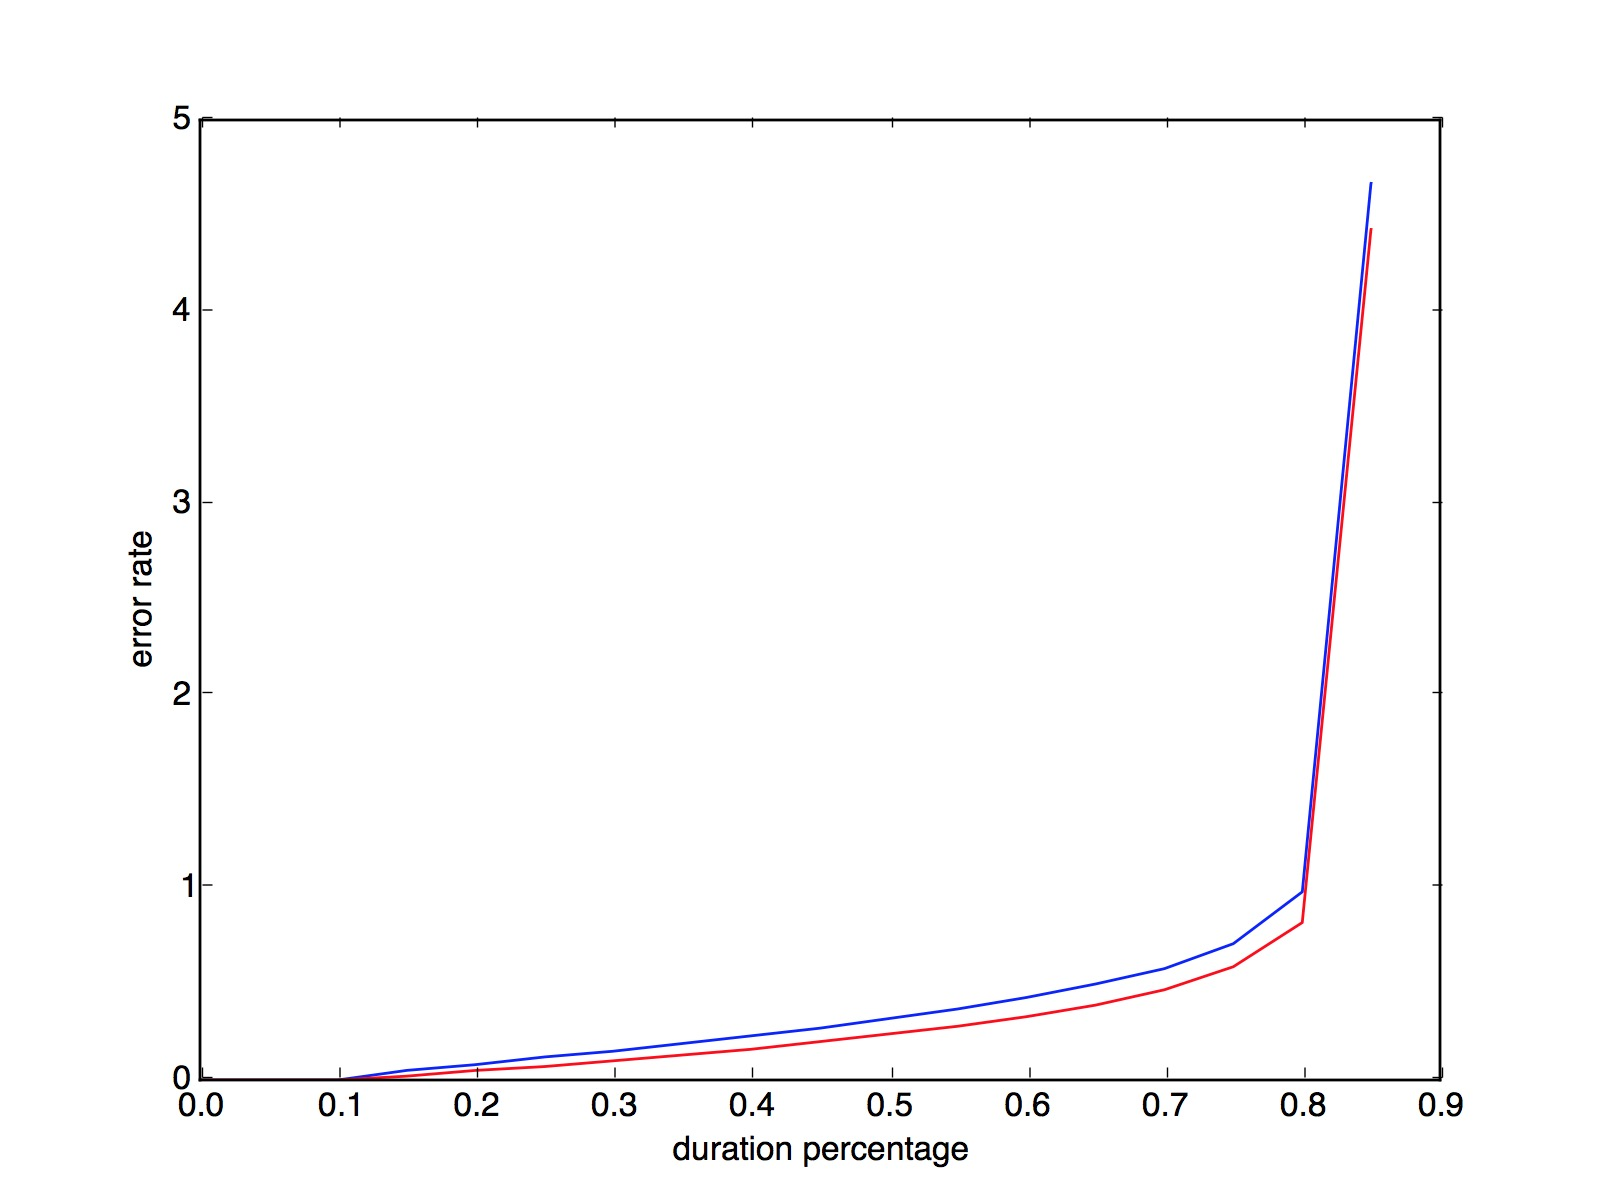
\includegraphics[scale=0.2]{wmerpmeram0s1} 
%\centering
%\end{figure}

%\begin{figure}
%\caption{Graph of PMER and WMER from transcription align, provided by MGB.}
%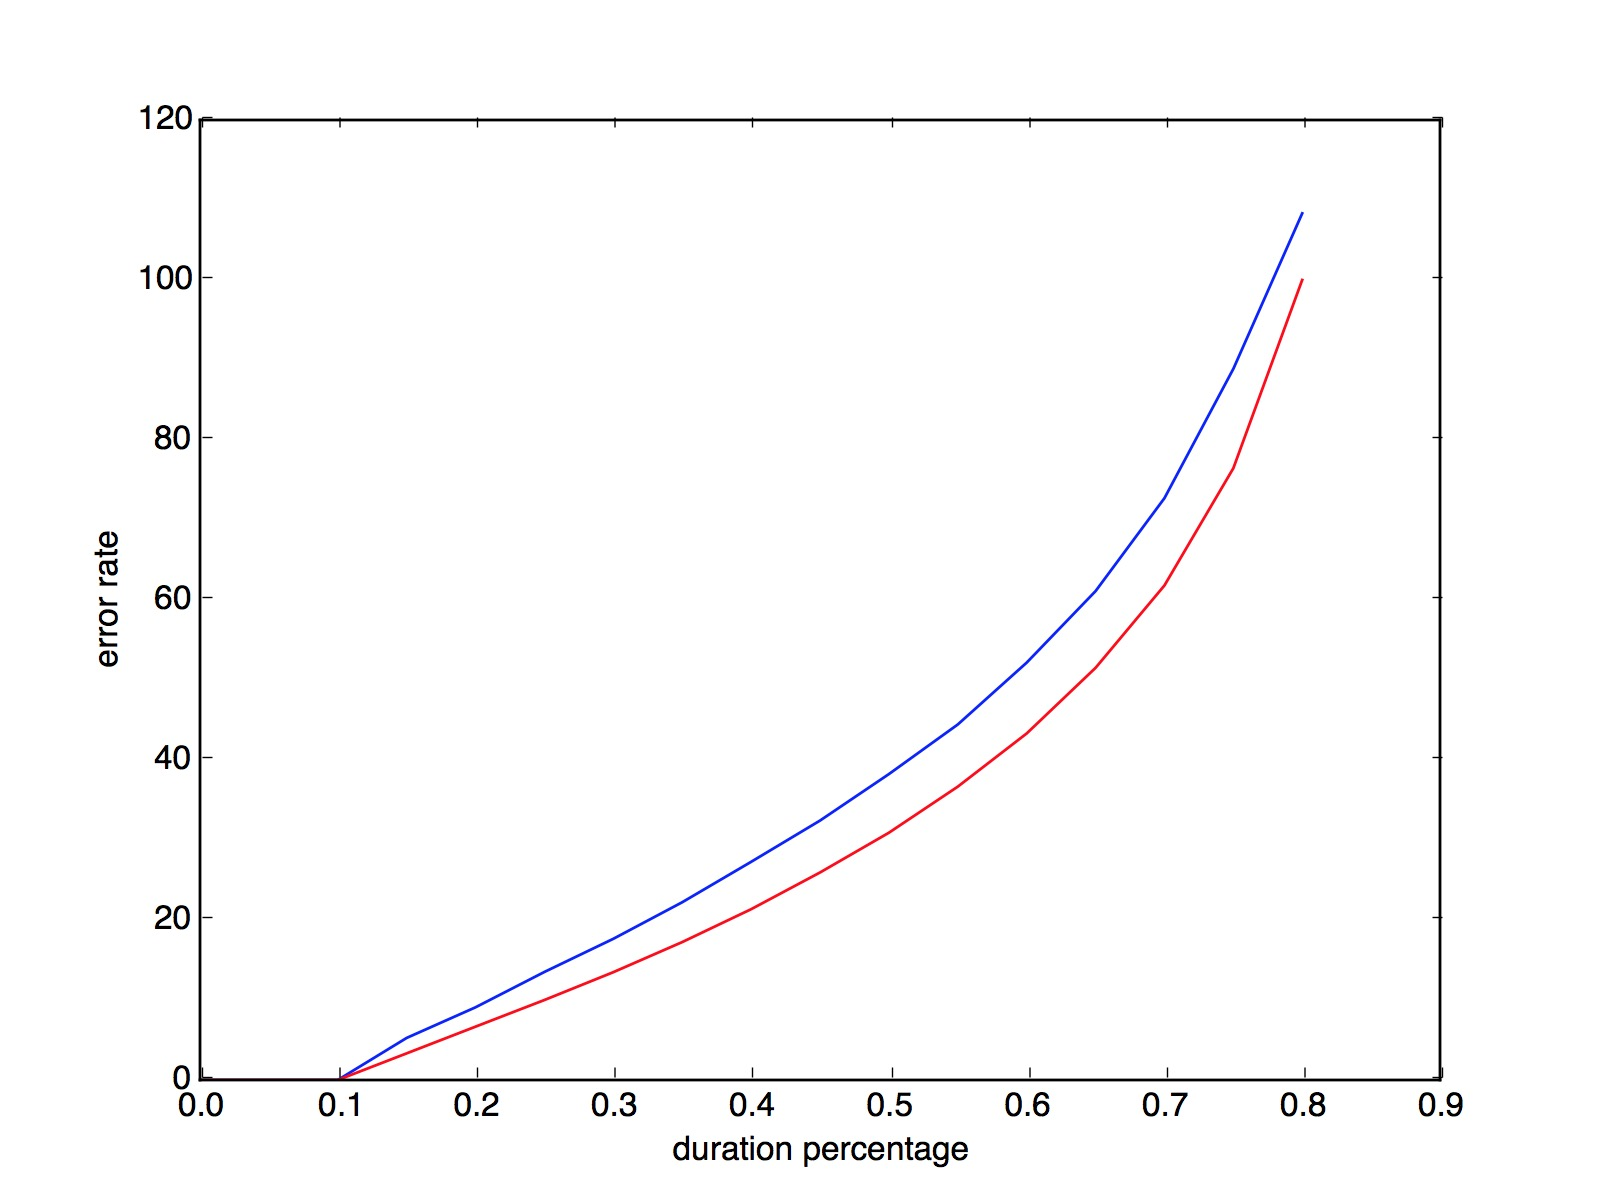
\includegraphics[scale=0.2]{wmerpmeram0align}
%\centering
%\end{figure}

%\subsubsection{Training acoustic model AM.100-v2}
%\begin{center}
%\begin{tabular}{ | c | c | c | c |  c |  }
%\hline
%\textbf{No.} & \textbf{Description} & \textbf{Result} & \textbf{execution time} & \textbf{extra info} \\ \hline \hline
%1 & GMM-V2\_decode &  & 2h 56m 41s & 20 hosts \\  \hline
%2 & TDNN-V2\_decode &  & 23h 52m 58s & 3 hosts \\  \hline
%\end{tabular}
%\end{center}


\section{Comparison}

Comparison between different speech recognizer:
\begin{center}
\label{wmerAM0s1}
\begin{tabular}{ | c | c | c |  c | c |  }
\hline
\textbf{No.} & \textbf{Acoustic model} & \textbf{Language Model}  &  \textbf{PER}  & \textbf{WER}  \\ \hline \hline
1 & TDNN.100  & LM.7weeks+subtitles.limited.1e-9 & 35.8  & 43.9 \\ 
& & Lexicon.7weeks+subtitles  & & \\ \hline


2 & TDNN.100-v1\_decode   & LM.7weeks+subtitles.limited.1e-9  & 34.3    & 42.3 \\
&  & Lexicon.7weeks+subtitles & & \\ \hline

3 & TDNN.100-v1   & LM.7weeks+subtitles.limited.1e-9  & 33.8   & 41.2 \\
&  & Lexicon.7weeks+subtitles & & \\ \hline


4 & TDNN.100-v2   & LM.7weeks+subtitles.limited.1e-9  & 33.3    & 40.5 \\
&  & Lexicon.7weeks+subtitles & & \\ \hline

5 & TDNN.100-v3   & LM.7weeks+subtitles.limited.1e-9  & 33.3    & 40.5 \\
&  & Lexicon.7weeks+subtitles & & \\ \hline
\end{tabular}
\end{center}


\begin{figure}
\caption{Average word duration}
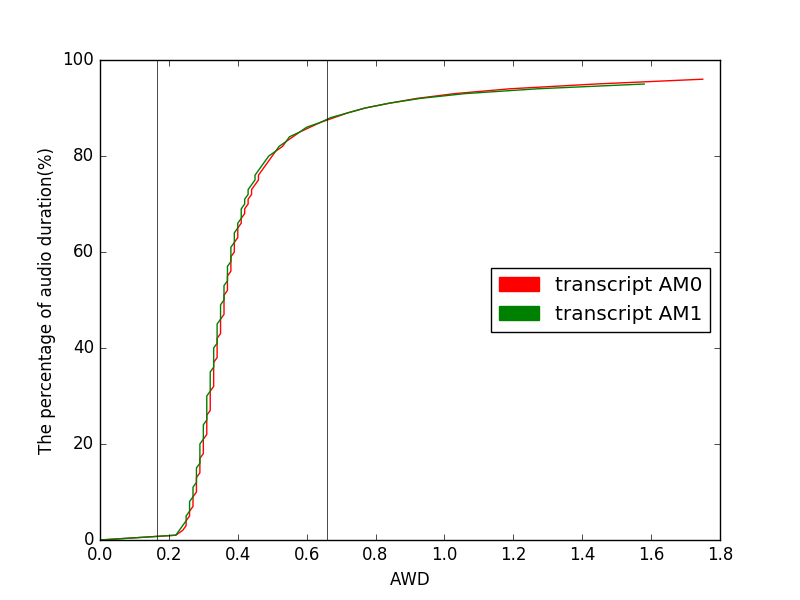
\includegraphics[scale=0.7]{awdLineChart}
\centering
\end{figure}

\begin{figure}
\caption{Phone match error rate}
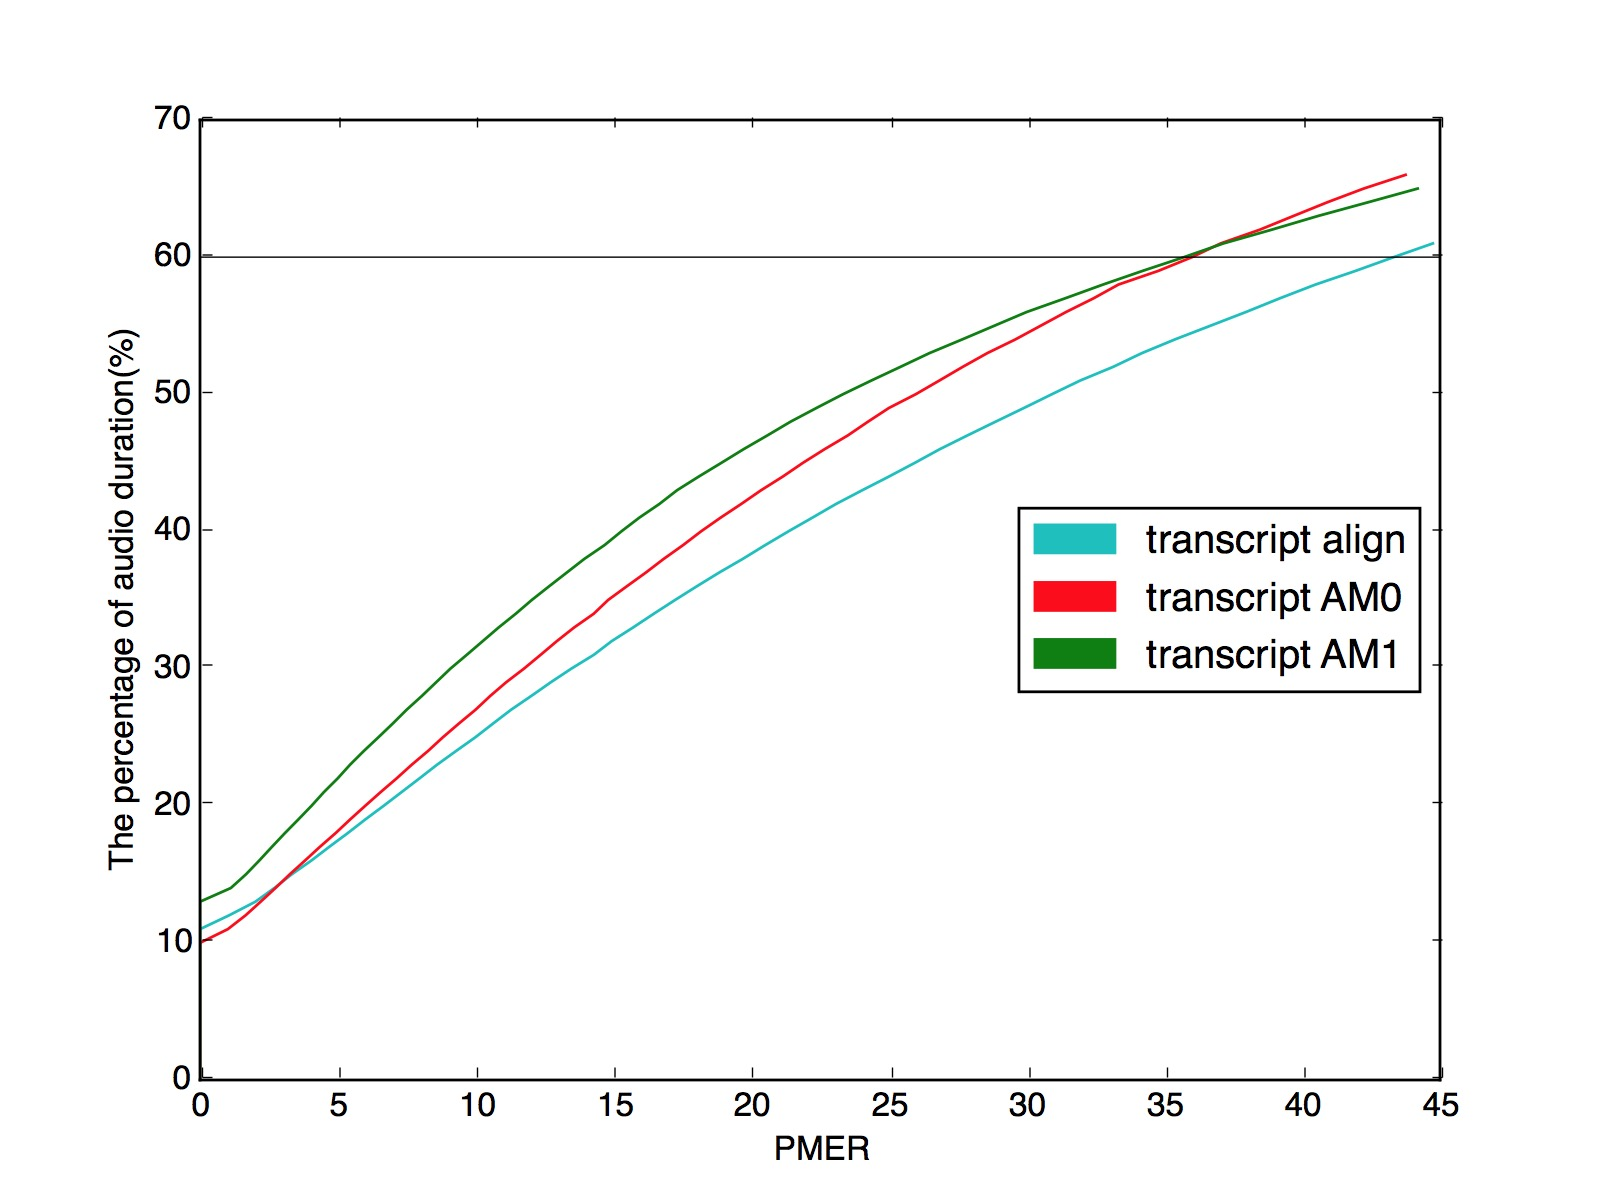
\includegraphics[scale=0.3]{pmerLineChart}
\centering
\end{figure}

\begin{figure}
\caption{Word match error rate}
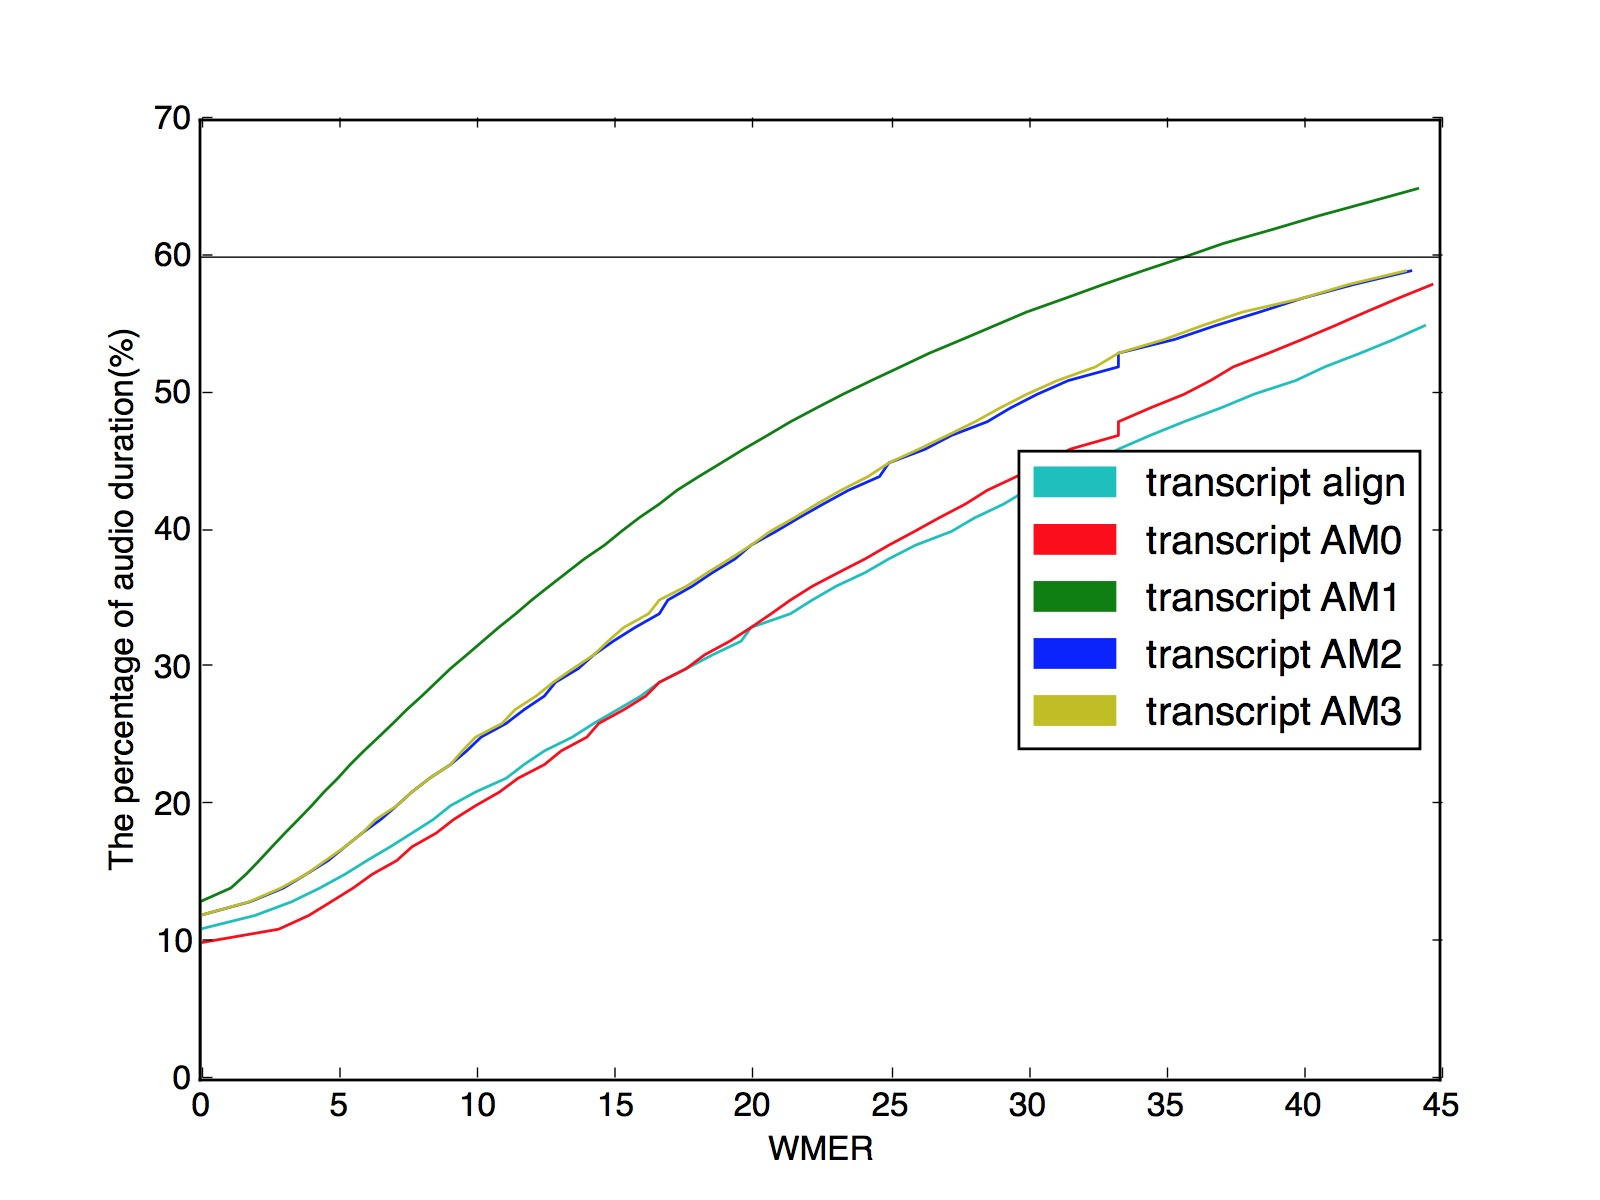
\includegraphics[scale=0.25]{wmerLineChart}
\centering
\end{figure}




%PER 32.2 | 9118 204786 | 75.0 10.0 15.0 7.2 32.2 82.7 | -1.058 | |
%WER 49.3 | 9118 64248 | 59.0 25.1 15.9 8.2 49.3 83.7 | -0.822 | |

%AM0_s1
%WMER
%[0, 0.05001182297101408, 0.1000055705823501, 0.15002999947778156, 0.20000377990423135, 0.250006911717846, 0.3000083202847346, 0.350008061797726, 0.4000080655439148, 0.45000218777410367, 0.5000070802963298, 0.5500076834326855, 0.6000113209817511, 0.6500022214898035, 0.7000031243212423, 0.7500004870045146, 0.8000498093227562, 0.8500152732106541]
%[0, 0.0, 0.0, 0.05, 0.08, 0.12, 0.15, 0.19, 0.23, 0.27, 0.32, 0.37, 0.43, 0.5, 0.58, 0.71, 0.98, 4.67]

%PMER
%[0, 0.05000255115439209, 0.10000343525488571, 0.15000458158857732, 0.20000319924500873, 0.2500218028172682, 0.3000072338900607, 0.3500012437345947, 0.4000032891535333, 0.45000364878763255, 0.5000033341077957, 0.5500060913025576, 0.6000314567451253, 0.6500026335705453, 0.700001251226977, 0.7500149847541436, 0.8000220313347739, 0.8500007005372576]
%[0, 0.0, 0.0, 0.02, 0.05, 0.07, 0.1, 0.13, 0.16, 0.2, 0.24, 0.28, 0.33, 0.39, 0.47, 0.59, 0.82, 4.43]

%Align
%WMER
%([0, 0.050002832118532126, 0.10000931677088468, 0.15000742869186362, 0.20000679558600154, 0.2500274408310134, 0.30000118379557716, 0.3500026485552931, 0.40000639849001596, 0.4500279240893308, 0.5000118004938804, 0.5500090133296115, 0.6000040159141051, 0.6500046752432919, 0.7000030681284111, 0.7500003184260248, 0.800006522114234], [0, 0.0, 0.0, 5.26, 9.09, 13.51, 17.65, 22.22, 27.27, 32.43, 38.24, 44.44, 52.17, 61.11, 72.73, 88.89, 108.33], 'b-'

%PMER
%[0, 0.05001950265750902, 0.10000225520549781, 0.15000134113549585, 0.20000690797165727, 0.25000294075800095, 0.30001437037921774, 0.35000064434442896, 0.40001250477732614, 0.45001977612927163, 0.5000107890229769, 0.5500005656744683, 0.60003347968693, 0.6500121301584764, 0.7000086499493287, 0.7500019667489803, 0.800000340903153], [0, 0.0, 0.0, 3.33, 6.67, 10.0, 13.48, 17.24, 21.35, 25.94, 30.91, 36.67, 43.32, 51.52, 61.82, 76.47, 100.0], 'r-'

